% Section content template for individual Educative lessons
% This file contains the actual content for a specific section
% Generated from Educative API section content

% Section: Background of Object-oriented Programming (OOP)
% Section ID: 6098172273491968
% Section Slug: background-of-object-oriented-programming-oop
% Generated: 2025-12-16T12:48:38.305321

\subsection{Definition}\label{0RryV0M1Xm0wMXNGtxGjw}
\\
We use programming to solve real-world problems, and it won't make much sense if one can't model real-world scenarios using programming languages. This is where object-oriented programmingcomes into play. \textbf{Object-oriented programming}, also called OOP, is a programming model that is dependent on the concept of \emph{objects} and \emph{classes}.
\\
OOP is a programming style, not a tool, so despite being old, it's vastly popular and established. This programming style involves dividing a program into pieces of objects that can communicate with each other. Every object has its own unique set of properties. These properties are later accessed and modified through the use of various operations.
\\
Check out the illustration below. It shows a real-life example of an employee record, where every employee can be considered an ``object''. Since every employee has a \emph{name}, \emph{age}, \emph{salary}, and \emph{designation}, all these can be considered as the properties of each employee.

\begin{figure}[htbp]
 \centering
 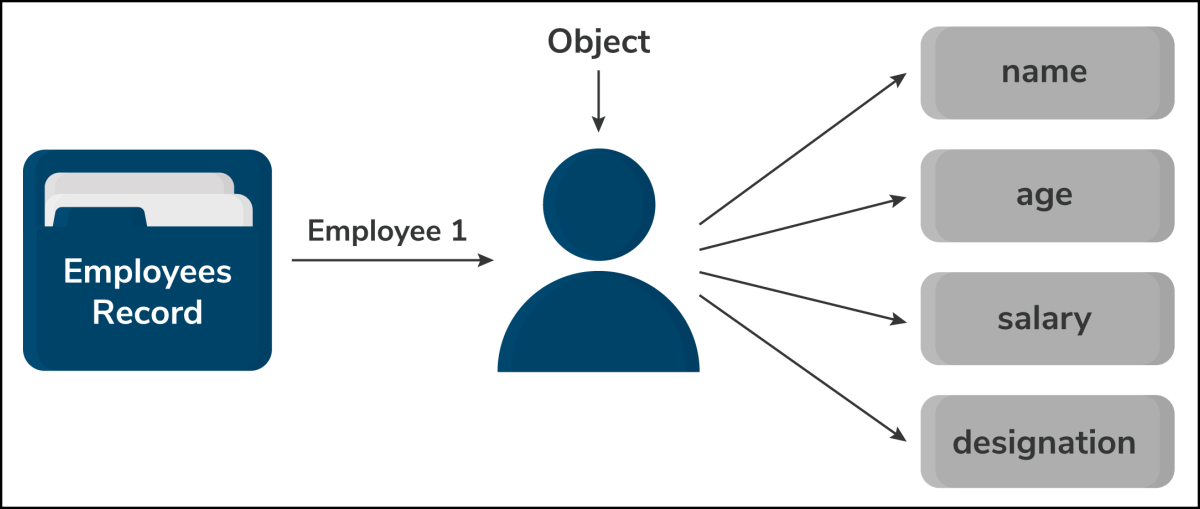
\includegraphics[width=0.5\textwidth]{Images/chapter_2/section_6098172273491968/6258836220674048.png}
 \caption{Real-life example of an employee record}
\end{figure}

\subsection{Building blocks of OOP}\label{PhVO7ftyPdT2DAdtGjcq_}
\\
The following are the essential concepts of object-oriented programming:

\begin{itemize}
\item
\protect\phantomsection\label{_irvYqogfrvSAwGx2RpUc}
Attributes
\item
\protect\phantomsection\label{QLRuYJSDHFYjTbYgjLawR}
Methods
\item
\protect\phantomsection\label{Ff4tPwqPtJ8PJ3DB4EzJJ}
Classes
\item
\protect\phantomsection\label{_AS90ohAU7UOVL2H2ICDq}
Objects
\end{itemize}

\subsubsection{Classes and objects}\label{TDWP5nWhfPpY4eTAkO1J2}
\\
In the real world, we can find many objects around us like cars, buildings, and humans. \emph{What are the characteristics of these objects?} All these objects have some \emph{state} and \emph{behavior}.
\\
Let\textquotesingle s take an example of a calculator. It has a state, i.e., either it is \emph{on} or \emph{off}. It also has behaviors, i.e., we can perform addition, subtraction, multiplication, division, and many other operations on numbers. Therefore, we can say that \textbf{objects} have state(s) and behavior(s).
\\
Interesting, isn't it? However, the question is, ``\emph{where do the objects come from?}''
\\
The answer to the question above is \textbf{classes}. A \textbf{class} can be thought of as a \emph{blueprint} for creating objects.

\subsubsection{Attributes}\label{qRUBeFf0Qka-h__x2lN25}
\\
Attributes are variables that represent the state of the object. In other words, if you were to implement the calculator object below in a computer program, variables could represent its state.

\subsubsection{Methods}\label{aIn8XDigrwLdNy_NPYT8Z}
\\
Methods are like functions that represent the behavior of the object. In other words, if you were to implement the calculator object below in a computer program, functions could represent its behavior. Methods have access to a class\textquotesingle s attributes (and other methods). They can accept parameters, return values, and are used to perform an action on an object of a class.
\\
The illustration below shows what a \texttt{Calculator} class should look like:

\begin{figure}[htbp]
 \centering
 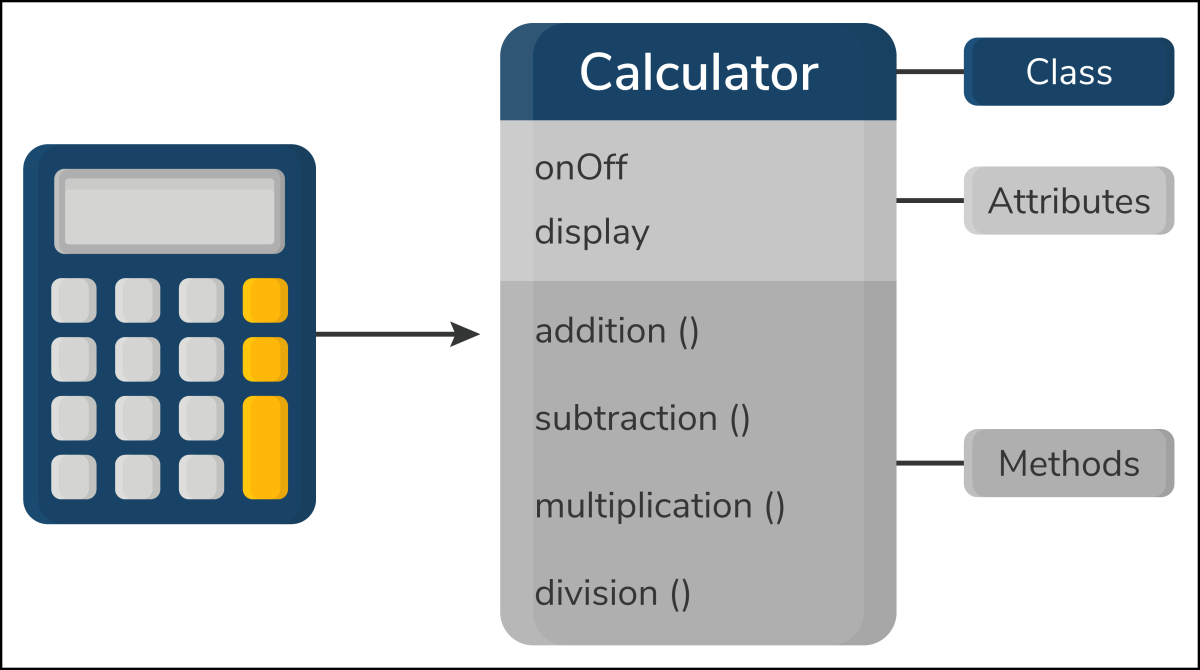
\includegraphics[width=0.5\textwidth]{Images/chapter_2/section_6098172273491968/5863675547353088.png}
 \caption{Calculator class with attributes and methods}
\end{figure}

\subsection{Principles of OOP}\label{PSdHLgXANdpN6aO6CG6cJ}
\\
The following are the four principles of object-oriented programming:

\begin{itemize}
\item
\protect\phantomsection\label{YfP29jG9J1DkAiMI7w5-1}
Encapsulation
\item
\protect\phantomsection\label{zxQgT31vDB6P4WAggCQm1}
Abstraction
\item
\protect\phantomsection\label{P1rHVVDbmABNB0VJuV_xs}
Inheritance
\item
\protect\phantomsection\label{blt9jcyzT3RDUM6nbvVEI}
Polymorphism
\end{itemize}
\\
In the next few lessons, we will explain these four principles in detail.

% End of section content